% Appendix (excluded from the 4-page main-text limit by the course spec).
% Every number below is copied from the committed CSVs in results/; regenerate with
% the commands in Section 4.3.
\section{Convergence and optimality checks (Role B)}\label{app:convergence}

Table~\ref{tab:convergence} is the bonus check: the iteration
$F^{(t+1)}=\alpha SF^{(t)}+(1-\alpha)Y$ versus the direct solution of
$(I-\alpha S)F=(1-\alpha)Y$, computed independently in
\texttt{experiments/convergence\_check.py}. Configuration: 200-point two-moons
toy, Gaussian coordinate noise $0.1$, one revealed label per class,
$\sigma=0.1$, stopping when $\lVert F^{(t+1)}-F^{(t)}\rVert_\infty<10^{-12}$.
These are our choices, not the paper's (the paper leaves the toy bandwidth
unstated), so the table is a qualitative reproduction of the paper's Figure~2 rather
than a
replication of their numbers.

\begin{table}[h]\centering\small
\caption{Iteration against closed-form solve. Zero argmax mismatches at every
$\alpha$; $F(0)$-independence measured from three different starts.}
\label{tab:convergence}
\begin{tabular}{lrrrrrr}
\toprule
$\alpha$ & $\max|\lambda(S)|$ & iters & predicted $\tfrac{\ln\mathrm{tol}}{\ln\alpha}$ &
$\lVert F_{\text{iter}}-F_{\text{solve}}\rVert_\infty$ & $F(0)$-independence & toy acc. \\
\midrule
0.5   & 1.0 &    29 & 40 & $8.1\times10^{-13}$ & $1.7\times10^{-12}$ & 0.77 \\
0.9   & 1.0 &   167 &   263  & $8.2\times10^{-12}$ & $1.6\times10^{-11}$ & 0.88 \\
0.95  & 1.0 &   326 &   539  & $1.7\times10^{-11}$ & $3.5\times10^{-11}$ & 0.94 \\
0.99  & 1.0 & 1{,}405 & 2{,}750 & $9.1\times10^{-11}$ & $1.9\times10^{-10}$ & 0.97 \\
0.999 & 1.0 & 10{,}860 & 27{,}618 & $7.5\times10^{-10}$ & $1.7\times10^{-9}$ & 1.00 \\
\bottomrule
\end{tabular}
\end{table}
\begin{figure}[ht]
  \centering
  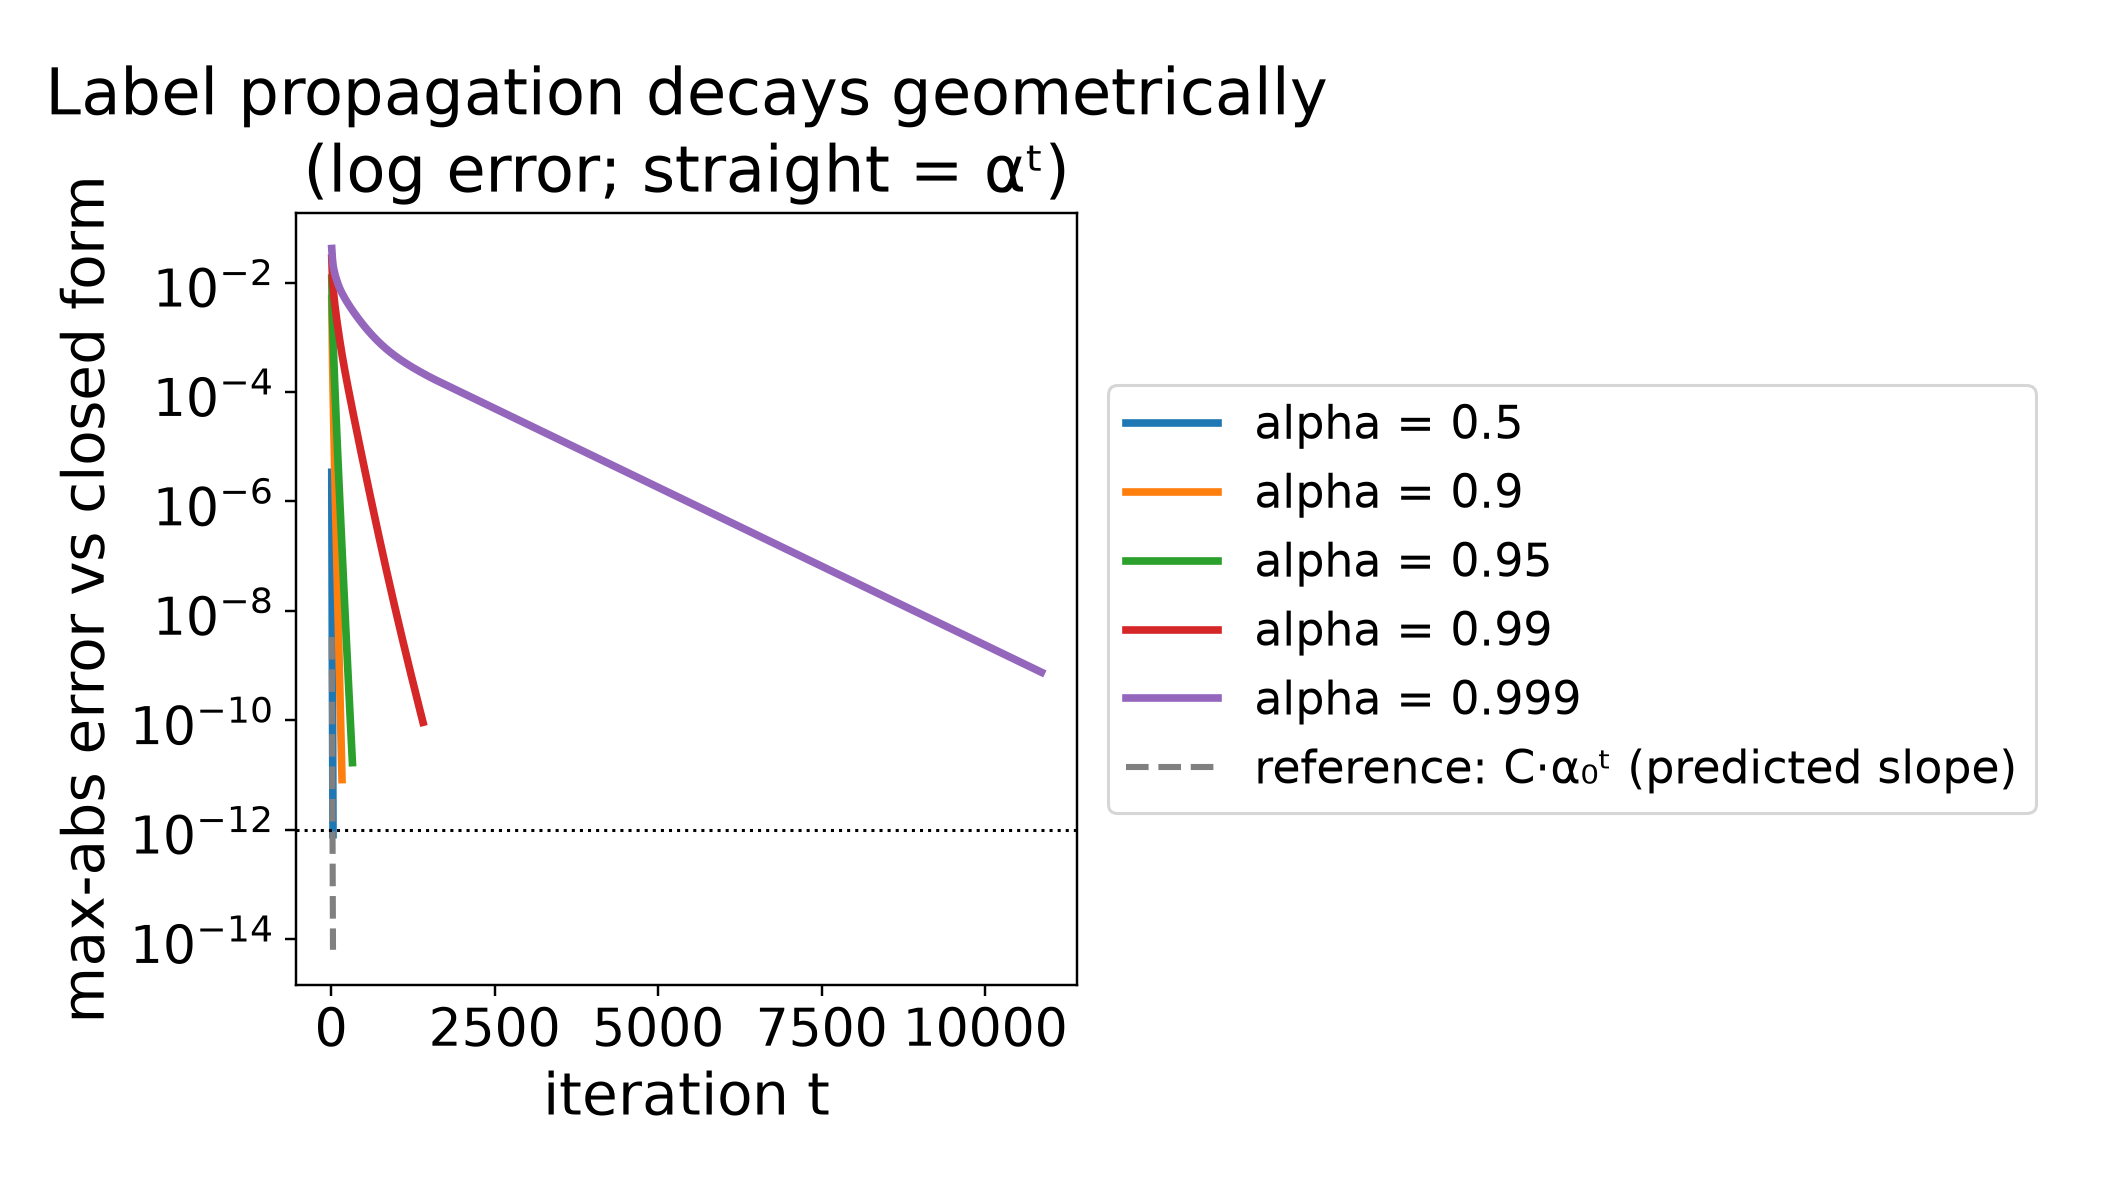
\includegraphics[width=0.50\linewidth]{figs/convergence_rate_big.png}
  \caption{Log max-abs error of the iteration against the closed form, for four
  values of $\alpha$, on our generated two-moons data. Straight lines confirm the
  geometric decay; the dashed line is the predicted $\alpha_0^{t}$ rate. Our
  result, not the paper's.}
  \label{fig:rate}
\end{figure}

\noindent
Two readings matter.
First, the stopping error is $\mathrm{tol}/(1-\alpha)$, not $\mathrm{tol}$, because
the residual carries the extra $(1-\alpha)$ factor --- observed
$9.1\times10^{-11}$ against the predicted $10^{-10}$ at $\alpha=0.99$, and
$7.5\times10^{-10}$ against $10^{-9}$ at $\alpha=0.999$: the contraction analysis
predicts its own stopping error. Second, the empirical decay slope is slightly
steeper than $\ln\alpha$ (e.g.\ $-0.0132$ vs $-0.0101$ at $\alpha=0.99$), so the
worst-case bound is valid but not tight here; the $\lambda=1$ eigenmode, the
degree-weighted constant $D^{1/2}\mathbf{1}$, nearly cancels for these starts.
The regularised objective $\mathcal{Q}(F)$ of the paper's Eq.~4 is confirmed at
$F^{*}$: stationarity residual $2.1\times10^{-17}$ with $\mu=(1-\alpha)/\alpha$,
and 18/18 random perturbations of $F^{*}$ increased $\mathcal{Q}$.

\section{Equation audit of the paper's operator variants}\label{app:variants}

Table~\ref{tab:variants} records the same check on the alternative normalisations
($P=D^{-1}W$). Relative gaps are matrix norms; the last column is how many of the
200 toy predictions change versus the main $S$-based argmax.

\begin{table}[h]\centering\small
\caption{Section~2/4 identities at $\alpha=0.99$ (\texttt{results/variants\_audit.csv}).
The printed transpose identity fails as algebra while the classification survives.}
\label{tab:variants}
\begin{tabular}{lcc}
\toprule
Claim under test & relative gap & argmax shift \\
\midrule
$(I-\alpha P)^{-1}Y=(D-\alpha W)^{-1}DY$ & $1.05\times10^{-15}$ & 6/200 \\
$(I-\alpha P^{\top})^{-1}Y=(D-\alpha W)^{-1}DY$ \emph{(as printed)} & $0.819$ & 6/200 \\
$(I-\alpha P^{\top})^{-1}Y=D(D-\alpha W)^{-1}Y$ \emph{(corrected)} & $1.36\times10^{-15}$ & 6/200 \\
Section~4 variant as written: $(D-\alpha W)^{-1}Y$ vs $(I-\alpha P^{\top})^{-1}Y$ & $0.828$ & 6/200 \\
Main $S$-based vs $(I-\alpha P)^{-1}Y$ (positive row scaling) & $0.330$ & 6/200 \\
\bottomrule
\end{tabular}
\end{table}

\section{Full bandwidth sweep and reference check}\label{app:sweep}

\begin{figure}[ht]
  \centering
  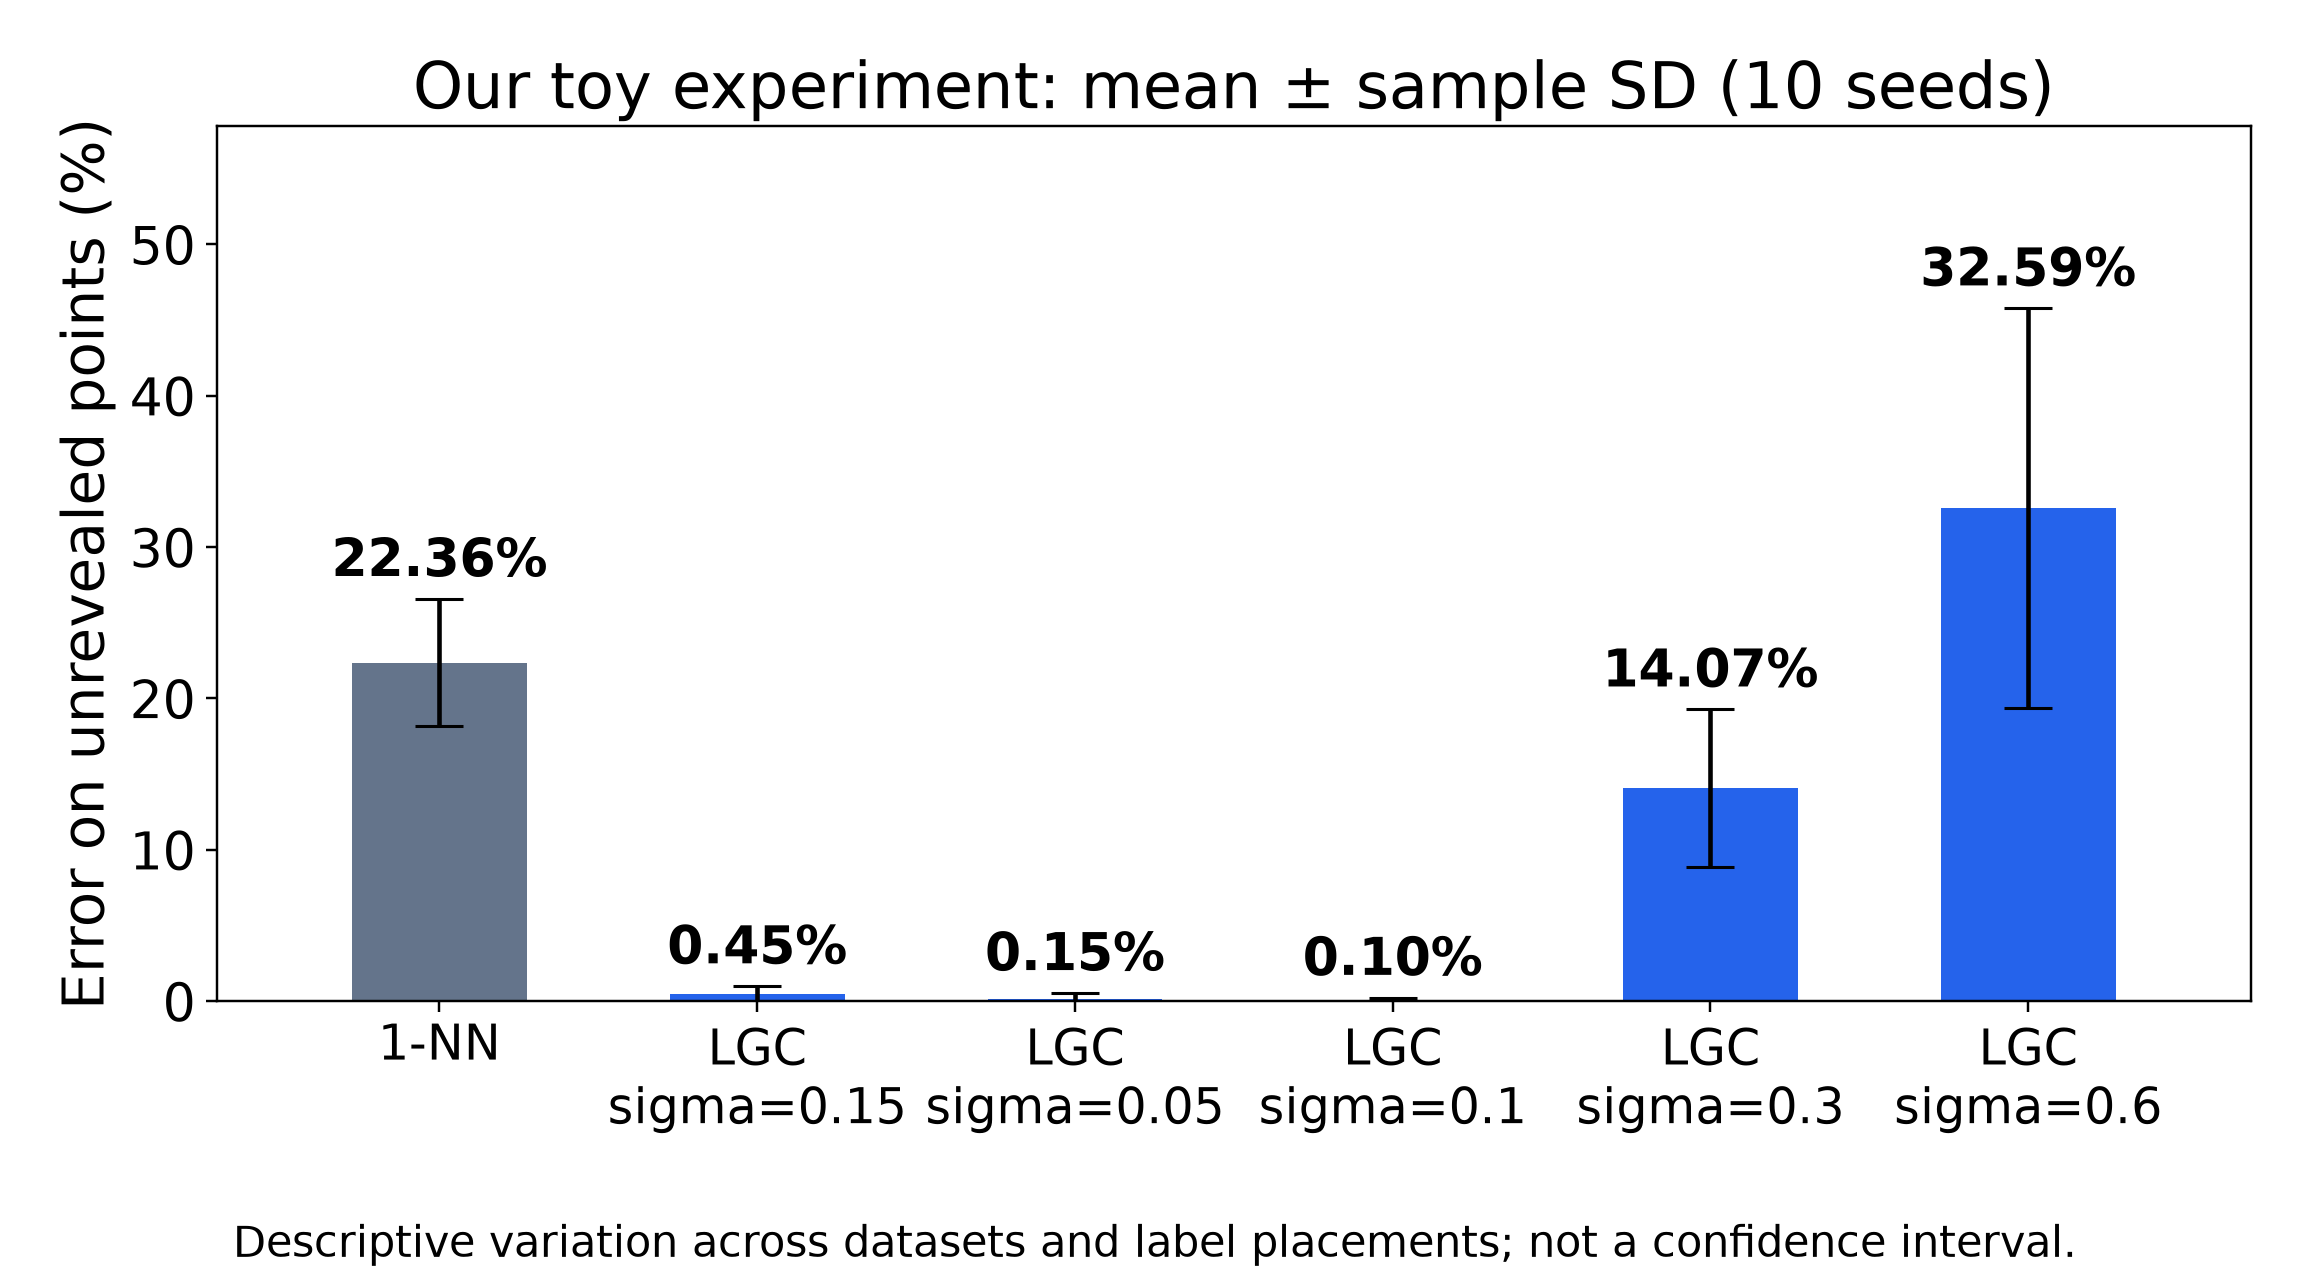
\includegraphics[width=0.58\linewidth]{figs/error_summary_big.png}
  \caption{Mean error per seed for LGC at five bandwidths against the 1-NN
  baseline on our ten fixed two-moons trials; bars are the sample SD across
  seeds. Our result, not the paper's.}
  \label{fig:errors}
\end{figure}

\begin{table}[h]\centering\small
\caption{Two-moons comparison, ten fixed seeds, $n=400$, noise $0.08$, one revealed
label per class, $\alpha=0.99$, evaluation on unrevealed labels only
(\texttt{results/comparison/summary.csv}, \texttt{paired.csv}). SD is the sample SD
across seeds, not a confidence interval. ``$>$1-NN'' counts paired trials where LGC
had lower error.}
\label{tab:sweep}
\begin{tabular}{lccc}
\toprule
Method & $\sigma$ & mean error (SD) & paired trials $>$ 1-NN \\
\midrule
1-NN & --- & 22.36\% (4.22) & --- \\
LGC & 0.05 & 0.15\% (0.40) & 10/10 \\
LGC & 0.10 & 0.10\% (0.13) & 10/10 \\
LGC & 0.15 & 0.45\% (0.54) & 10/10 \\
LGC & 0.30 & 14.07\% (5.21) & 10/10 \\
LGC & 0.60 & 32.59\% (13.20) & 2/10 \\
\bottomrule
\end{tabular}
\end{table}

The sweep is descriptive: bandwidths were declared before the run and every trial is
retained, including the two at $\sigma=0.60$ where 1-NN wins. Separately,
B's closed-form reference was run through C's exact protocol
(\texttt{experiments/convergence\_check.py --protocol},
\texttt{results/protocol\_check.csv}): mean unlabelled accuracy $99.55\%$ over the ten
seeds, 1{,}263--1{,}314 iterations to tolerance (worst-case prediction 2{,}750), maximum
deviation from the direct solve $8.27\times10^{-11}$, and zero argmax mismatches against
A's merged predictor on all ten seeds. That reference is what let us treat C's 1-NN
numbers as a fair comparison rather than an unverified baseline.
